\UseRawInputEncoding
%
% Module 1 Programming Discussion
% CSC160-C00: Computer Science I (C++)
% Author: Ashton Hellwig
%


\documentclass[a4paper, 11pt]{article}
  % Packages
  \usepackage[latin1,utf8]{inputenc}  % Encoding
  \usepackage[english]{babel}         % Internationalization
  \usepackage{times}                  % Times New Roman font
  \usepackage{soul}                   % Highlighting
  \usepackage{hyperref}               % Links (internal and external)
  \usepackage{fancyhdr}               % Headers and footers
  \usepackage[dvipsnames]{xcolor}     % Text Colors
  \usepackage{listings}               % Code Snippets
  \usepackage[section]{algorithm}     % For TOC support
  \usepackage{algpseudocode}          % Algorithmic notation environments
  \usepackage{enumitem}               % Ordered lists
  \usepackage{geometry}               % Page layout
  \usepackage{graphicx}               % Image support
  \usepackage[toc, page]{appendix}    % Appendix
  \usepackage{setspace}               % Paragraph and line spacing
  \usepackage{bookmark}               % Required for appendix
  \usepackage{adjustbox}              % Required for appendix
  \usepackage{csquotes}               % Required for appendix
  \usepackage{amsthm}                 % Theorem environments
  \usepackage{array}                  % Arrays
  \usepackage{makecell}               % Table helpers
  \usepackage{amsmath}                % Mathematical symbols
  \usepackage{amssymb}                % Misc. symbols for logic and math
  \usepackage{relsize}                % Relative Sizing
  \usepackage{multicol}               % Multi-figure displays (grid)
  \usepackage{etoolbox,refcount}      % Required for mdframed
  \usepackage{parcolumns}             % Paragraph grids
  \usepackage{mdframed}               % Colored box environments
  \usepackage{siunitx}                % Typesetting measurements and currency
  \usepackage[                        % Bibliography management
    backend=biber,%
    style=apa%
  ]{biblatex}

  % Bibliography Setup
  \addbibresource{main.bib}
  \newcommand{\CiteSection}[2]{%
    (\autocite{#1}, ~\S {#1})%
  }

  % Typesetting measurements and currency
  \sisetup{%
    group-four-digits=true,%
    group-separator={,}
  }
  \newcommand{\usd}[1]{\SI{#1}[\$\ensuremath{\,}]{}}

  % Tables
  \renewcommand\theadalign{bc}
  \renewcommand\theadfont{\bfseries}
  \renewcommand\theadgape{\Gape[4pt]}
  \renewcommand\cellgape{\Gape[4pt]}

  % Lists
  \newcounter{countitems}
  \newcounter{nextitemizecount}
  \newcommand{\setupcountitems}{%
    \stepcounter{nextitemizecount}%
    \setcounter{countitems}{0}%
    \preto\item{\stepcounter{countitems}}%
  }
  \makeatletter
  \newcommand{\computecountitems}{%
    \edef\@currentlabel{\number\c@countitems}%
    \label{countitems@\number\numexpr\value{nextitemizecount}-1\relax}%
  }
  \newcommand{\nextitemizecount}{%
    \getrefnumber{countitems@\number\c@nextitemizecount}%
  }
  \newcommand{\previtemizecount}{%
    \getrefnumber{countitems@\number\numexpr\value{nextitemizecount}-1\relax}%
  }
  \makeatother
  \newenvironment{AutoMultiColItemize}{%
  \ifnumcomp{\nextitemizecount}{>}{3}{\begin{multicols}{2}}{}%
  \setupcountitems\begin{itemize}}%
  {\end{itemize}%
  \unskip\computecountitems\ifnumcomp{\previtemizecount}{>}{3}{\end{multicols}}{}}



  % Colors
  \newcommand{\commentstylecolor}{\color{Gray}}
  \newcommand{\keywordstylecolor}{\color{MidnightBlue}}
  \newcommand{\stringstylecolor}{\color{ForestGreen}}
  \newcommand{\questioninput}{\color{Red}}
  \newcommand{\answertcolor}{\color{Green}}
  \newcommand{\myanswer}{\answertcolor{\hl}}

  % Symbols
  \newcommand{\answerflow}{\rotatebox[origin=c]{180}{$\Lsh$}}
  \newcommand{\toanswer}{\mathlarger{\mathlarger{\answerflow}}\quad}

  % Math
  \newcommand{\highlight}[1]{%
    \colorbox{green!50}{$\displaystyle#1$}}

  % Image Directory
  \graphicspath{ {screenshots/} }


  % Hyperlink Setup
  \hypersetup{
    colorlinks = true,
    urlcolor = blue,
    linkcolor = blue
  }


  % Algorithm Settings
  \newcommand{\pluseq}{\mathrel{{+}{=}}}
  \newcommand{\minuseq}{\mathrel{{-}{=}}}


  % Syntax-Highlighting for Code Snippets
  \lstset{
    backgroundcolor=\color{white},
    breaklines=true,%
    captionpos=b,%
    frame=tlrb,%
    tabsize=2,%
    numbers=left,%
    showstringspaces=false,%
    commentstyle=\commentstylecolor,%
    keywordstyle=\keywordstylecolor,%
    stringstyle=\stringstylecolor%
  }
  \lstset{literate=
  {á}{{\'a}}1 {é}{{\'e}}1 {í}{{\'i}}1 {ó}{{\'o}}1 {ú}{{\'u}}1
  {Á}{{\'A}}1 {É}{{\'E}}1 {Í}{{\'I}}1 {Ó}{{\'O}}1 {Ú}{{\'U}}1
  {à}{{\`a}}1 {è}{{\`e}}1 {ì}{{\`i}}1 {ò}{{\`o}}1 {ù}{{\`u}}1
  {À}{{\`A}}1 {È}{{\'E}}1 {Ì}{{\`I}}1 {Ò}{{\`O}}1 {Ù}{{\`U}}1
  {ä}{{\"a}}1 {ë}{{\"e}}1 {ï}{{\"i}}1 {ö}{{\"o}}1 {ü}{{\"u}}1
  {Ä}{{\"A}}1 {Ë}{{\"E}}1 {Ï}{{\"I}}1 {Ö}{{\"O}}1 {Ü}{{\"U}}1
  {â}{{\^a}}1 {ê}{{\^e}}1 {î}{{\^i}}1 {ô}{{\^o}}1 {û}{{\^u}}1
  {Â}{{\^A}}1 {Ê}{{\^E}}1 {Î}{{\^I}}1 {Ô}{{\^O}}1 {Û}{{\^U}}1
  {œ}{{\oe}}1 {Œ}{{\OE}}1 {æ}{{\ae}}1 {Æ}{{\AE}}1 {ß}{{\ss}}1
  {ű}{{\H{u}}}1 {Ű}{{\H{U}}}1 {ő}{{\H{o}}}1 {Ő}{{\H{O}}}1
  {ç}{{\c c}}1 {Ç}{{\c C}}1 {ø}{{\o}}1 {å}{{\r a}}1 {Å}{{\r A}}1
  {€}{{\euro}}1 {£}{{\pounds}}1 {«}{{\guillemotleft}}1
  {»}{{\guillemotright}}1 {ñ}{{\~n}}1 {Ñ}{{\~N}}1 {¿}{{?`}}1
}
  \newenvironment{alltt}{\ttfamily}{\par}
  \lstMakeShortInline[language=c++,columns=fixed]|


  % Page Configuration
  %% Style
  \pagestyle{fancy}

  %% Layout
  \geometry{%
    a4paper,%
    top=2.5cm,%
    bottom=2.5cm,%
    left=2.5cm,%
    right=2.5cm%
  }
  \setlength{\headheight}{15pt}
  \setlength{\floatsep}{12pt}
  \setlength{\parindent}{0.5em}
  \setlength{\parskip}{0.5em}
  \renewcommand{\baselinestretch}{0.75}

  %% Title page
  \title{%
    Module 1 Programming Discussion\\%
    \large{Topic Goes Here}
  }
  \author{Ashton Hellwig}
  \date\today
  \setcounter{tocdepth}{3}

  %% Subsequent pages
  \lhead{CSC160}
  \rhead{Computer Science I (C++)}
  \lfoot{M1C1HW}
  \rfoot{A. Hellwig}

  % MDFramed Config
  \mdfdefinestyle{AnswerFrame}{%
    linecolor=black,
    outerlinewidth=4pt,
    roundcorner=20pt,
    innertopmargin=4pt,%
    innerbottommargin=4pt,%
    innerrightmargin=4pt,%
    innerleftmargin=4pt,%
    leftmargin = 4pt,%
    rightmargin = 4pt,%
    backgroundcolor=green!20%
  }

% Document Content
\begin{document}
  % Title Page
  \maketitle
  \tableofcontents
  \listofalgorithms
  %\lstlistoflistings
  \newpage

  \section{Initial Post}
    \subsection{Prompt:}
      Chapter 2 Programming Exercise 16 \parencite[~\S2-16c]{textbook}.
      \begin{mdframed}[style=AnswerFrame,nobreak=true,align=center]
        A milk carton can hold \SI{3.78}{\liter} of milk. Each morning, a dairy
          farm ships cartons of milk to a local grocery store. The cost of
          producing one liter of milk is \usd{0.38}, and the profit of each
          carton of milk is \usd{0.27}. Write a program that does the following:

        \begin{enumerate}[label=\alph*.]
          \item Prompts the user to enter the total amount of milk produced in
            the morning.
          \item Outputs the number of milk cartons needed to hold milk.
            (Round your answer to the nearest integer.)
          \item Outputs the cost of producing milk.
          \item Outputs the profit for producing milk.
        \end{enumerate}
      \end{mdframed}

    \subsection{Initial Post}
      Below is the code snippet used to create the solution to \textit{Chapter
        2`s Programming Exercise 16} \parencite[~\S2-16c]{textbook}. The snippet
        for |general_functions::pauseprompt();| is also included as an
        alternative to |system('pause');|. The source header file is attached
        and displayed below.

      \begin{lstlisting}[%
        language=c++,%
        columns=fixed,%
        caption={main.cc}
      ]
//===--------------------------------------------------------
///
/// \file
/// This file contains the main function to run the program.
///
//===-------------------------------------------------------

#include <iostream>

using namespace std;

/**
 * \brief Prompts the user to press <RET> to continue running the program.
 *
 * \return int Exit code.
 */
int pauseprompt(); // Prototype
int pauseprompt() {
  std::cout << "Press enter to continue..." << '\n';
  std::cin.ignore();

  return 0;
}

int main() {
  // Declaring Variables
  double cartonMaxVolume =
      0.00;                   /** Maximum amount of milk per carton in liters */
  double cartonProfit = 0.00; /** Profit from one carton of milk */
  double literCost = 0.00;    /** Cost of producing one liter of milk */
  double totalMilkProduced = 0.00; /** Amount of liters of milk produced */
  double totalCost = 0.00;         /** Cost of producing all of the milk */
  double totalProfit = 0.00;       /** Total profit earned */
  int numberOfCartonsNeeded =
      0; // Cartons needed to hold amount of milk produced

  // Assigning values to variables
  cartonMaxVolume = 3.78000;
  cartonProfit = 0.27000;
  literCost = 0.38;

  // Prompting user to enter amount of milk produced
  cout << "Please enter the total amount of milk produced in the morning in "
          "liters (L): ";
  cin >> totalMilkProduced;

  // Multiply the cost of milk with the number of cartons for total cost.
  totalCost = literCost * totalMilkProduced;

  // Calculating total cartons produced
  numberOfCartonsNeeded = static_cast<int>(totalMilkProduced / cartonMaxVolume);

  // Calculating total profit
  totalProfit = static_cast<double>(cartonProfit * numberOfCartonsNeeded);

  // Number of milk cartons needed to hold the milk
  cout << "You will need " << numberOfCartonsNeeded
       << " cartons to hold the milk you have produced." << '\n';

  // Cost of production
  cout << "Cost of producing " << totalMilkProduced << "L of milk: $"
       << totalCost << '\n';

  // Profit
  cout << "Profit from producing " << totalMilkProduced << " ("
       << numberOfCartonsNeeded << " cartons) of milk: $" << totalProfit
       << endl;

  // "Press enter to continue"
  pauseprompt(); // `system("pause")` does not work on Linux.

  return 0;
}
      \end{lstlisting}


      \subsubsection{Image of Compilation \& Running}
        An image is included below to show the program compiling and then
          running.
        \begin{figure}[H]
          \centering
          \caption{Chapter 2 Programming Exercise 16 Solution Image}
          \label{lst:soln}
          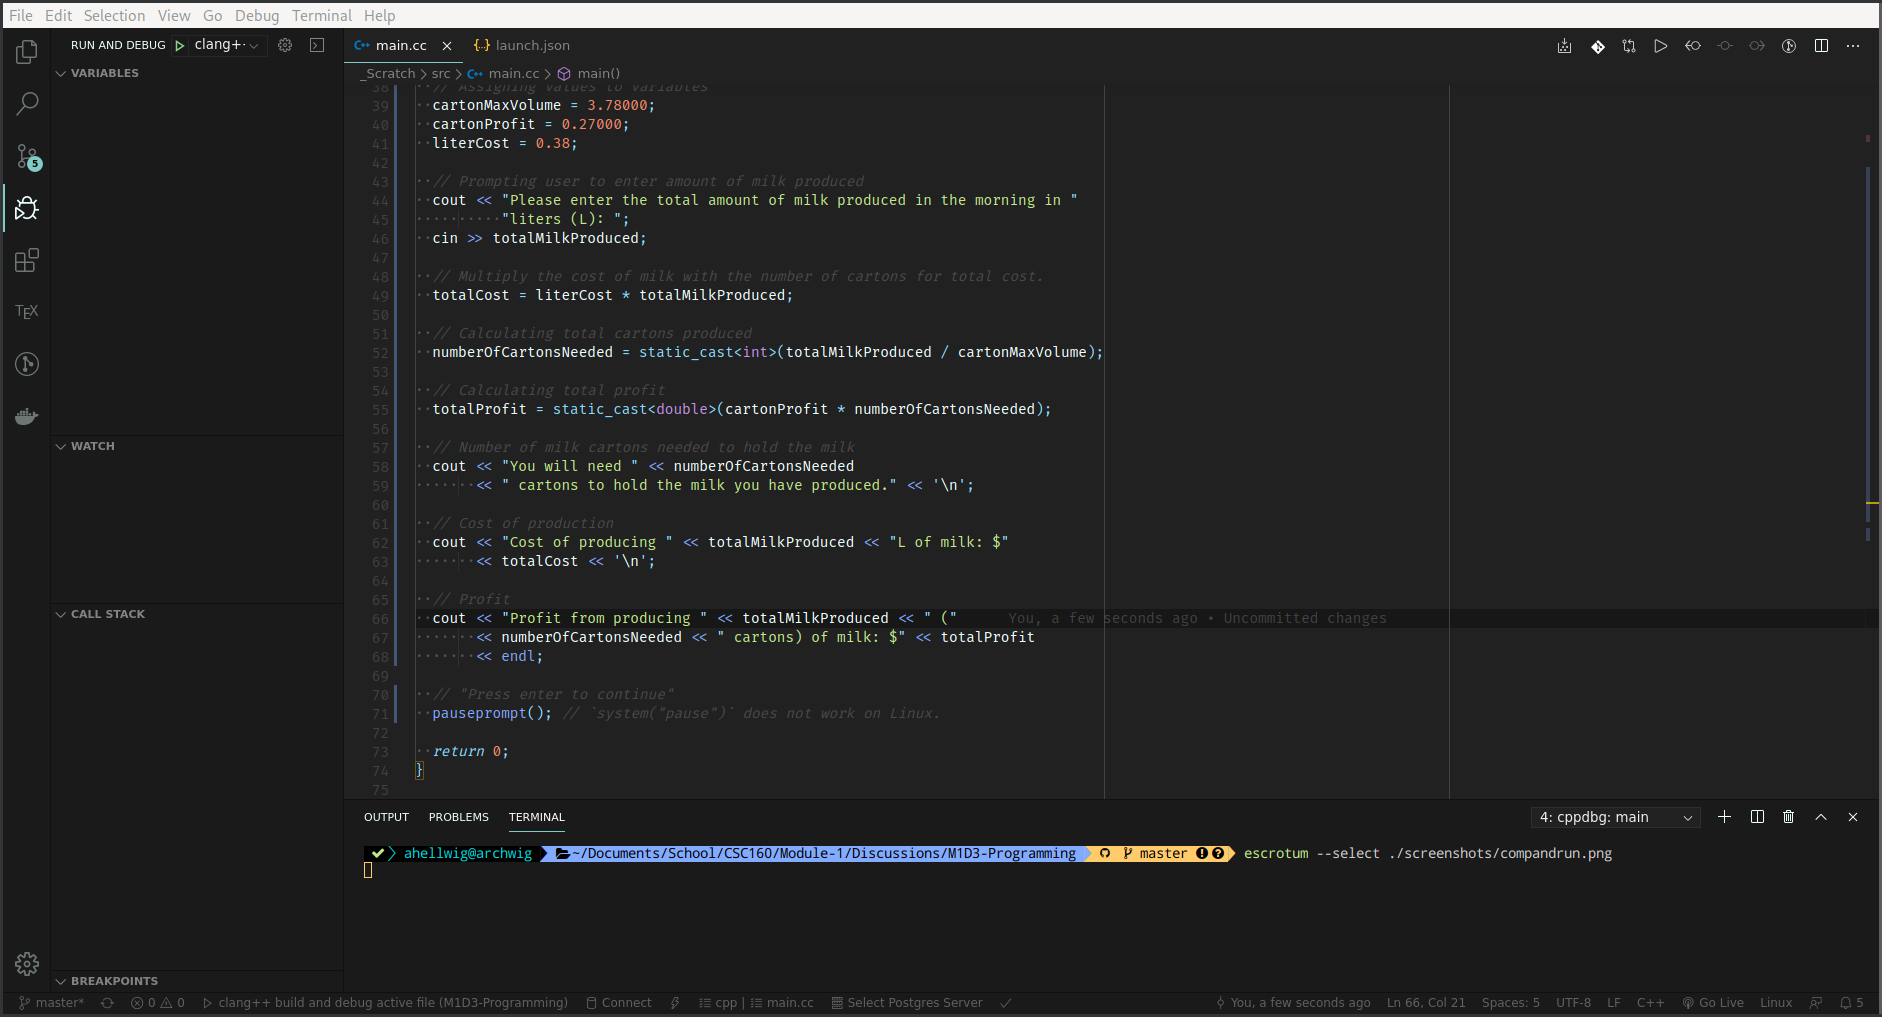
\includegraphics[width=\textwidth]{compandrun.png}
        \end{figure}

  % Bibliography
  \newpage
  \printbibliography[%
    heading=bibintoc,%
    title={Works Consulted}%
  ]
\end{document}
